% NEW
% + Argument for soundness and completeness of recognition by derivatives

% + Exhaustive battery af positive/negative examples on challenging grammars
%   run through the implementation

% + Alternative definition of derivative: fully equational

% + Refined complexity argument

% + Derivatives and zippers



% TODO:

% + Include better comparison to Danielsson in related work.

% + Include explanation of test grammar, test input.

% + Expand discussion of define/fix. 

% + Identify language as Racket up front.

% + Mark Scala and Haskell implementations "deprecated."

% + Mark Racket implementation as standard reference implementation.

% + Discuss how \delta can be seen as an operator on languages or handled with
%   a conditional and immediate evaluation during the derivative.

%   - try to be more consistent about using \delta as the property or the language
%     Specifically, look at section 5.3 "Step 3: Fixed Points". \delta the
%     property is used as an example, but we promised to only use it as a
%     language from now on...

%   - We actually need to continue to use \delta?, the boolean variant which is
%     computed via fixed-point.  It's used for determining if a delta node is
%     "essentially-epsilon".  delta is essentially epsilon if the argument
%     language is nullable.

% + (for David) drop references to Kleene algebra and regular algebra and stick
%   with regular expression and context-free grammar.  It will make life easier.

% + It's still unfortunate that \circle is used for both grammar concatentation
%   and function composition (see compaction section)

%   Matt:  Maybe we just live with this for now, and think about fixing for camera-ready.

\newcommand{\cat}{\mathrel{\circ}}

\newcommand{\nullability}{\delta}

\newcommand{\downto}{\downarrow}

\newcommand{\full}[1]{\lfloor #1 \rfloor}

\newcommand{\ttempty}{$\emptyset$}
\newcommand{\ttdelta}{$\updelta$}
\newcommand{\ttepsilon}{$\upepsilon$}

\newcommand{\ttepstar}{$\upepsilon$\mbox{\tt *}}
\newcommand{\ttepsred}{$\upepsilon\downarrow$}


%\newcommand{\ttcup}{U}
\newcommand{\ttcup}{{\footnotesize\ensuremath{{\cup}}}}
\newcommand{\ttcirc}{$\mathtt{\circ}$}
\newcommand{\ttstar}{$\mathtt{\star}$}
\newcommand{\ttred}{{{\tt →}}}
%\newcommand{\ttred}{$\mathtt{\rightarrow}$}

\newcommand{\ttlb}{\mbox{\tt\{}}
\newcommand{\ttrb}{\mbox{\tt\}}}



\section{Introduction}


It is easy to lose sight of the essence of parsing.
%
Implementation details like forbidden grammars, shift-reduce conflicts and
opaque action tables distract from the principle task: the conversion of
input strings into parse trees.
%
Brzozowski's derivative ends the distraction.
%
It enables a clean,
straightforward and equational connection between an input string, a grammar
and the resulting parse trees.



Brzozowski formulated the derivative in the context of regular expressions to
create a straightforward equational theory for recognizing regular
languages~\cite{mattmight:Brzozowski:1964:Derivative}.
%
Yet, the theory of the derivative applies--with modest generalization--to
context-free languages as well.
%
When gently tempered with laziness, memoization and fixed points, an
implementation of Brzozowski's derivative extends directly to a purely
functional technique for generating parse forests from arbitrary context-free
grammars.
%
Despite its seemingly impossible simplicity, the derivative transparently handles
ambiguity, left-recursion, right-recursion, ill-founded recursion and any
combination thereof.
%
No special handling of any of these cases is required.


\subsection{Outline}

\begin{itemize}

\item 
After a review of formal languages we introduce Brzozowski's derivative for
regular languages.  A brief implementation highlights its robust elegance.

\item 
As our implementation of the derivative engages context-free languages,
non-termination emerges as a problem.

\item 
Three small, surgical modifications to the implementation (but not the
theory)---laziness, memoization and fixed points---guarantee termination.
%
Recovering termination empowers the derivative to recognize arbitrary
context-free languages.

\item
Since the modifications are small, we construct an argument for the
soundness and completeness of the derivative as applied to context-free
languages.

\item
We supplement our soundness and completeness argument with a sequence of
increasingly challenging examples to build intuition
for the effectivess of the derivative of context-free grammars.

\item 
We generalize the derivative to parsers and parser combinators through an
equational theory for generating parse forests.

\item 
We find naive parsing with derivatives gives poor performance in both theory
and practice.
%
An analysis of the structure of grammers as they transform through the
derivative highlights room for improvement.
% The root cause is vestigial structure left in the grammar by earlier
% derivatives. This structure is malignant; though it no longer serves a purpose
% it still grows in size with each derivative.

\item 
To correct the poor performance of the the naive parsing theory we develop an
optimization---compaction---which collapses grammars by trimming excess mass.
%
Like the derivative, compaction also comes from a clean equational theory and
its implementation exploits laziness, memoization and fixed points.

\item
Further analysis shows that while practical parsing times are recovered through
compaction, there is still grammar structure to be exploited for performance.
%
Through yet another equational theory we develop a second
optimization---focusing---which when coupled with compaction recovers linear
parse times for a wide array of sensible grammars.


\end{itemize}
%
In this article we provide code in Racket. The implementation approach adapts
readily to other functional languages.
%
All code and test cases within or referenced from this article
are available from: \begin{center}
\texttt{http://www.ucombinator.org/projects/parsing/} \end{center}



\section{Preliminary: Formal languages}

A language $L$ is a set of strings.
%
A string $w$ is a sequence of characters from an alphabet $A$.
%
% (From a parser's perspective, a ``character'' might be a token/terminal from an
% input stream.)
%
%We'll use the \texttt{typewriter font} to denote literal strings.


Two atomic languages arise often in formal languages: the empty language and
the null (or empty-string) language:
%
\begin{itemize}
\item
The empty language $\emptyset$ contains no strings at all:
\begin{equation*}
 \emptyset = \set{}
 \text.
\end{equation*}

\item
The null language $\epsilon$ contains only the length-zero ``null'' string:
\begin{equation*}
 \epsilon = \set{ w } \text{ where } \mathit{length}(w) = 0
 \text.
\end{equation*}
%
Or, using C notation for strings, $\epsilon = \set{\mbox{\tt ""}}$.
%
For convenience we may use the symbol $\epsilon$ to refer to both the null language and the null string. 
%
That is, depending on the context $\epsilon = \set{\mbox{\tt ""}}$ or $\epsilon = \mbox{\tt ""}$.

\end{itemize}
%
Given an alphabet $A$ there is a singleton language for every character $c$ in that alphabet.
%
Where it is clear from context we use the character itself to denote that language; that is:
\begin{equation*}
 c \equiv \set{ c }
 \text.
\end{equation*}


\subsection{Operations on languages}
Because languages are sets, set operations like union apply:
\begin{equation*}
  \set{\tt foo} \union \set{{\tt bar}, {\tt baz}} = 
  \set{{\tt foo}, {\tt bar}, {\tt baz}}
  \text.
\end{equation*}
%
Language concatenation $(\cat)$ lifts string concatenation to the product of
the two languages:
%
\begin{equation*}
  L_1 \cat L_2 =
  \setbuild{ w_1 w_2 }{ w_1 \in L_1 \text{ and } w_2 \in L_2 }
  \text.
\end{equation*}
%
The $n$th power of a language is the set of strings of $n$ consecutive words
from that language:
\begin{align*}
  L^0 &= \epsilon
  \\
  L^n &= \setbuild{ w_1w_2 \ldots w_n }{ w_i \in L} 
  \text.
\end{align*}
%
The non-empty repetition of a language (its Kleene star) is the infinite union
of all its powers:
\begin{equation*}
  L^\star = \bigcup_{i = 0}^\infty L^i
  \text.
\end{equation*}
%


\subsection{Regular languages and context-free languages}
A \emph{regular language} is 
the composition of atomic languages over union, concatenation and
repetition.
%
Allowing mutually recursive definitions in a regular language yields exactly
the set of \emph{context-free languages} under a least-fixed-point
interpretation.
%
The mutually recursive equations that define such a language correspond to a 
\emph{context-free grammar}.
%
For instance, given the language $L$:
\begin{align*}
  L &= (\set{\tt x} \cat L)
    \union \epsilon
  \text.
\end{align*}
%
The least-fixed-point interpretation of $L$ is the set of all finite-length
sequences of the character x, including the null string.
%
(The greatest-fixed-point interpretation of $L$ would include an infinite
string of {\tt x}'s.)


Kleene star becomes syntactic sugar for recursive union and concatenation in
context-free grammars:
%
\begin{align*}
   L^\star = L'\text{, where }
   L' = (L \cat L') \union \epsilon
   \text.
\end{align*}


\subsection{Encoding languages}
To represent the structure of regular expressions in code we define a
\texttt{struct} for each kind of language:
\begin{code}
(define-struct \ttempty     \ttlb\ttrb)        
(define-struct \ttepsilon     \{\})   
(define-struct token \{value\})    

(define-struct \ttcup     \{this that\}) 
(define-struct \ttcirc     \{left right\})
(define-struct \ttstar     \{lang\})\end{code}


\begin{example}
%
In code, the language:
\begin{align*}
 L_{\mathit{ab}} &= L_{\mathit{ab}} \cat \set{{\tt a}, {\tt b}} 
 \\
 &\,\union \epsilon
 \text,
\end{align*}
becomes:
\begin{code}
(define L (\ttcup (\ttcirc L (\ttcup (token 'a) (token 'b)))
             (\ttepsilon)))\end{code}
\end{example}


\section{Brzozowski's derivative}
%
Brzozowski defined the derivative of regular expressions in his work
on the recognition of regular languages~\cite{mattmight:Brzozowski:1964:Derivative}.
%
The derivative of a language $L$ with respect to a character $c$, written
$D_c(L)$, is a new language which has been ``filtered'' and ``chopped'':
\begin{enumerate}

\item
First, retain only the strings in $L$ which start with $c$.

\item
Second, remove $c$ from the beginning of every string.

\end{enumerate}
%
Formally:
\begin{equation*}
  D_c(L) = 
  \setbuild{ w }{ cw \in L }
  \text.
\end{equation*}
%

\begin{example}
\begin{align*}
  &D_{\tt b}\set{{\tt foo}, {\tt bar}, {\tt baz}} = \set{{\tt ar}, {\tt az}}
  \\
  &D_{\tt f}\set{{\tt foo}, {\tt bar}, {\tt baz}} = \set{{\tt oo}}
  \\
  &D_{\tt a}\set{{\tt foo}, {\tt bar}, {\tt baz}} = \emptyset
  \text.
\end{align*}
\end{example}


\subsection{Recognition with the derivative}
%
The simplicity of the derivative's definition masks its power.
%
It is straightforward to determine the membership of a string within a language
through successive derivatives using the following property:
\begin{align*}
  cw \in L \text{ iff } w \in D_c(L)
  \text.
\end{align*}
%
To determine membership of string $s$ in language $L$, just derive $L$ with
respect to each character of $s$ in sequence.
%
The resulting language contains the null string if and only if $s$ is contained
in $L$.

\subsection{A recursive definition of the derivative}

Brzozowski showed that regular languages are
closed under the derivative.
%
A constructive implementation of the derivative for regular languages is
described recursively over the structure of regular expressions:
\begin{itemize}

\item
For the atomic languages:
\begin{align*}
  D_c(\emptyset) &= \emptyset
  \\
  D_c(\epsilon) &= \emptyset
  \\
  D_c(c) &= \epsilon
  \\
  D_c(c') &= \emptyset \text { if } c \neq c'
  \text.
\end{align*}

\item
For the derivative over union:
\begin{align*}
  D_c(L_1 \union L_2) &= D_c(L_1) \union D_c(L_2)
  \text.
\end{align*}

\item
The derivative over Kleene star ``peels off'' a copy of the language to derive:
\begin{align*}
  D_c(L^\star) &=
  D_c(L) \cat L^\star\!\!
  \text.
\end{align*}


\item
The derivative of concatenation must first consider the possibility that the
first language could be null:
\begin{align*}
 D_c(L_1 \cat L_2)  
 &= 
 D_c(L_1) \cat L_2 \text{ if } \epsilon \not\in L_1 
 \\
 D_c(L_1 \cat L_2)  
 &= 
 (D_c(L_1) \cat L_2)
  \union
 D_c(L_2)
 \text{ if } \epsilon \in L_1 
\end{align*}
%
Concatenation without a conditional can be expressed through the nullability
function: $\nullability$.
%
The nullability function returns the null language if its input language
contains the null string, and the empty set otherwise:
\begin{align*}
  \nullability(L) &= \emptyset \text{ if } \epsilon \not\in L
  \\
  \nullability(L) &= \epsilon \text{ if } \epsilon \in L
  \text.
\end{align*}
Concatentation is equivalently defined:
\begin{align*}
 D_c(L_1 \cat L_2)  
 &= 
 (D_c(L_1) \cat L_2)
  \union
 (\nullability(L_1) \cat D_c(L_2))
 \text.
\end{align*}


\end{itemize}


\subsection{Nullability of regular languages}
Conveniently, nullability may also be computed using structural recursion on
regular languages:
\begin{align*}
  \nullability(\emptyset) &= \emptyset
  \\
  \nullability(\epsilon) &= \epsilon
  \\
  \nullability(c) &= \emptyset
  \\
  \nullability(L_1 \union L_2) &= \nullability(L_1) \union \nullability(L_2)
  \\
  \nullability(L_1 \cat L_2) &= \nullability(L_1) \cat \nullability(L_2)
  \\
  \nullability(L^\star) &= \epsilon
  \text.
\end{align*}
%
A recursive implementation of the Boolean variant of the nullability function
is also straightforward:
\begin{code}
(define (\ttdelta? L)
  (match L
    [(\ttempty)         #f]
    [(\ttepsilon)         #t]    
    [(token _)   #f]

    [(\ttcup L1 L2)   (or  (\ttdelta? L1) (\ttdelta? L2))]
    [(\ttcirc L1 L2)   (and (\ttdelta? L1) (\ttdelta? L2))]
    [(\ttstar _)       #t])) \end{code}



\begin{example}
A couple examples illustrate the derivative on regular languages:

{
\small
\begin{align*}
 D_{\tt f}\set{{\tt foo},{\tt bar}}^\star &= 
 \set{\tt oo} \cat 
 \set{{\tt foo},{\tt bar}}^\star
 \\
 D_{\tt f}\set{{\tt foo},{\tt bar}}^\star \cat \set{\tt frak} &= 
 \set{\tt oo} \cat 
 \set{{\tt foo},{\tt bar}}^\star 
 \cat \set{\tt frak}
 \union
 \set{\tt rak}
 \text.
\end{align*}
}
%
\end{example}

% [David: TODO: we don't define null? at all, and we should in this section.
% This will also require modifying the "alternative-implementation" section]

% [Matt: TODO: null? is a built-in in Scheme. Resolved?]
% [David: TODO: Ah, yes, I must have thought this was grammar nullability :)]


\subsection{An implementation of the derivative}
Because the description of a regular language is not recursive, it is
straightforward to transliterate the derivative into working code:
\begin{code}
(define (D c L)
  (match L
    [(\ttempty)                     (\ttempty)]
    [(\ttepsilon)                     (\ttempty)]
    [(token a)               (if (equal? c a) (\ttepsilon) (\ttempty))]
    
    [(\ttcup L1 L2)               (\ttcup (D c L1) (D c L2))]
    [(\ttcirc (and (? \ttdelta?) L1) L2)  (\ttcup (D c L2) (\ttcirc (D c L1) L2))]
    [(\ttcirc L1 L2)               (\ttcirc (D c L1) L2)]
    [(\ttstar L1)                  (\ttcirc (D c L1) (\ttstar L1))]))\end{code}
%
%
Matching a regular language {\tt L} against a {\tt cons}ed list of
characters {\tt w} is straightforward:
\begin{code}
(define (matches? w L)
  (if (null? w)
      (\ttdelta? L)
      (matches? (cdr w) (D (car w) L))))\end{code}


\subsection{Aside: An alternative implementation} 
%
The nullability function $\delta$ admits an alternative and arguably more
elegant theory and implementation.
%
Rather than defining nullability as an operator on languages we define
nullability as a language combinator like {\tt \ttcup} or {\tt \ttcirc}.
%
\begin{code}
(define-struct \ttdelta \ttlb{}lang\ttrb)\end{code}
%
To fit $\delta$ into our existing framework for recognition we need only define the
derivative of nullability; the interpretation follows as before.
%
The derivative of nullability is always empty:
%
\begin{align*}
  D_c(\delta(L)) &= \emptyset
  \text.
\end{align*}

Conveniently, nullability of nullability is equal to nullability:
\begin{align*}
 \nullability(\nullability(L)) = \nullability(L)
 \text,
\end{align*}


Promoting nullability to a connective allows for a simpler definition of the
derivative; concatenation no longer requires a branch in logic:
%
\begin{code}
(define (D c L)
  (match L
    [(\ttempty)         (\ttempty)]
    [(\ttepsilon)         (\ttempty)]
    [(\ttdelta L)       (\ttempty)]
    [(token a)    (if (equal? c a) (\ttepsilon) (\ttempty))]

    [(\ttcup L1 L2)   (\ttcup (D c L1) (D c L2))]
    [(\ttcirc L1 L2)   (\ttcup (\ttcirc (D c L1) L2)
                    (\ttcirc (\ttdelta L1) (D c L2)))]
    [(\ttstar L1)      (\ttcirc (D c L1) (\ttstar L1))]))\end{code}

We will use this formulation of the derivative and nullability for the
remainder of the paper, as its simplicity will be of even greater
effect as we develop theories for parsing.

\section{Derivatives of context-free languages}
%
Before we discuss the derivative of context-free languages it must first be
established whether or not such a thing makes sense.
%
The derivative is a set-theoretic operation on languages and is \emph{not}
defined in terms of any particular language structure such as regularity.
%
Brzozowski showed---constructively---that regular expressions, and thus regular
languages, are closed under the derivative.
%
It remains for us to show that context-free grammars are closed under the
derivative, after which closure for context-free languages would directly
follow.
 
Fortunately the argument for closure of context-free grammars under the
derivative is trivial because context-free grammars are merely recursive
regular expressions.
%
The proofs of closure are the same.


Knowing that the derivative of context-free grammars follows the same elegant
theory as that of regular expressions we turn our attention to implementation.
%
Because a context-free grammar is a recursive regular expressions, it is
tempting to use the same code for computing the derivative.
%
From the perspective of parsing this has two chief drawbacks:
\begin{enumerate}
\item It doesn't work.  
\item It wouldn't produce a parse forest even if it did.
\end{enumerate}
The first problem comes from the recursive implementation of the derivative
running into the recursive nature of context-free grammars.
%
It quickly leads to non-termination.

The second comes from the fact that our regular implementation only
\emph{recognizes} whether a string is in a language rather than parsing the
string.
%
We tackle the termination problem in this section, 
and the parsing problem in a later section~(\ref{sec:parsing}).

\begin{example}
Consider the following left-recursive language:
\begin{align*}
  L &=  L \cat \set{\tt x} 
  \\
    &\,\union \epsilon
  \text.
\end{align*}
If we take the derivative of $L$ we get a new language:
\begin{align*}
  D_{\tt x}L &=  D_{\tt x}L \cat \set{\tt x} 
  \\
    &\,\union \epsilon
  \text.
\end{align*}
\end{example}
%
Mathematically this is sensible.
%
Computationally it is not (yet).
%
The code from the previous section recurs forever as it attempts to compute the
derivative of the language $L$.


\subsection{Step 1: Laziness} 
%
Preventing the implementation of the derivative from making an infinite descent
on a recursive grammar requires targeted laziness.
%
Specifically it requires making the fields of the structs {\tt \ttcup},
{\ttcirc} and {\ttstar} lazy.\footnote{%
  Lisp implementations that do not support lazy fields can provide them
  transparently with macros and mechanisms like {\tt delay} and {\tt force} or by caching thunks.
  Syntactic support for laziness is not essential to this implementation; it is
  merely a convenience.
}
%
With lazy fields the computation of any (potentially self-referential)
derivatives in those fields gets suspended until the values in those fields are
required.
%


\subsection{Step 2: Memoization}
%
With laziness we can repeatedly compute the derivative until the end of the
  recognition algorithm when it tests the resulting language for nullability.
%
Nullability currently walks (eagerly) the structure of the entire language and
fails to terminate on a derived language such as the one above.
%
We need the derivative to return a finite (if lazily explored) graph.
%
Memoizing the derivative will ``tie the knot'' when it re-encounters
a language it has already seen:

\begin{code}
(define/memoize (D c L)
  #:order ([L #:eq] [c #:equal])
  (match L
    [(\ttempty)                     (\ttempty)]
    [(\ttepsilon)                     (\ttempty)]
    [(token a)               (if (equal? c a) (\ttepsilon) (\ttempty))]

    [(\ttdelta L)                   (\ttempty)]
    [(\ttcup L1 L2)               (\ttcup (D c L1) (D c L2))]
    [(\ttcirc (and (? \ttdelta?) L1) L2)  (\ttcup (D c L2) (\ttcirc (D c L1) L2))]
    [(\ttcirc L1 L2)               (\ttcirc (D c L1) L2)]
    [(\ttstar L1)                  (\ttcirc (D c L1) (\ttstar L1))]))\end{code}
%
The  \texttt{define/memoize}
form above defines a derivative function \texttt{D} that memoizes first by pointer equality
on the language and then by value equality on the character.


\subsection{Step 3: Fixed points}
%
The computation of nullability%
\footnote{%
  We are still committed to presenting $\delta$ as a language-level connective
  rather than a property of a language, as mentioned in a previous section.
  %
  Here we consider the boolean variant, which will be needed to interpret the
  $\delta$ connective.
}
is more challenging than
the computation of the derivative because it isn't looking for a structure;
it's looking for a single answer: ``Yes, it's nullable,'' or ``No, it's not.''
%
As such, laziness and memoization can't help side-step self-dependencies 
the way they did for the derivative.
%
Consider the nullability of the left-recursive language $L$:
\begin{align*}
  \delta(L) &=  (\delta(L) \cat \emptyset)
    \union \epsilon
  \text.
\end{align*}
%
To know the nullability of $L$ requires knowing the nullability of $L$.
%
For decades this problem has been solved by interpreting the nullability of $L$
as the least fixed point of the nullability equations.

To expose only the essence of nullability we can hide the computation of a
least fixed point behind a purely functional abstraction: {\tt define/fix}.
%
Internally, the {\tt define/fix} form uses Kleene's theorem 
to compute the least fixed point of a monotonic recursive 
definition, and it allows the prior definition of nullability
to be used with little change:

\begin{code}
(define/fix (\ttdelta? L)
  #:bottom #f
  (match L 
    [(\ttempty)         #f]
    [(\ttepsilon)         #t]    
    [(token _)   #f]

    [(\ttdelta L)       (\ttdelta? L)]
    [(\ttcup L1 L2)   (or  (\ttdelta? L1) (\ttdelta? L2))]
    [(\ttcirc L1 L2)   (and (\ttdelta? L1) (\ttdelta? L2))]
    [(\ttstar _)       #t])) \end{code}
%
The \texttt{\#:bottom} keyword indicates from where to begin the iterative
ascent toward the least fixed point.
%
%\texttt{define/fix} monotonically refines this map using $\delta$ until
%it reaches a fixed point.

% [David: TODO: Matt, I'm not sure how to end "so that given an instance: ..." ]

The {\tt define/fix} form defines a function mapping nodes in a graph $(V,E)$
to values in a lattice $X$ so that given an instance of {\tt define/fix}:
\def\botX{{\bot_X}}
\begin{code}
(define/fix (\(f\) \(v\)) #:bottom \(\botX\) \(\mathit{body}\))\end{code}
%
after this definition the function $f : V \to X$ is a least fixed point:
\begin{equation*}
 f = \lfp(\lambda f . \lambda v . \mathit{body})
 \text,
\end{equation*}
which is easily computed with straightforward iteration:
\begin{equation*}
 \lfp(F) = F^n(\bot_{V \to X}) \text{ for some finite } n
 \text.
\end{equation*}


% \parapgraph{The fixed point of what?}
% %
% A least-fixed-point computation requires a monotonic function $F : X \to X$,
% and then finding the least $x$ such that $x = F(x)$.
% %
% With \texttt{define/fix}, this function $F$ is defined \emph{implicitly}.
% %
% The iteration-space ($X$) for the function $F$ in \texttt{define/fix} is a
% vector under a product ordering.
% %
% If the function defined explicitly by \texttt{define/fix} is $f : Y \to Y$,
% then $X = Y^*$.
% %
% In this case, $f = \delta$ and $Y = L$.
% %
% The function $F$ simply lifts $f$ across each component:
% 



\subsection{Recognizing context-free languages}
%
No special modification is required for the {\tt matches?} function.  
%
It works as-is for recognizing context-free languages.

With access to laziness, memoization and a library for computing fixed points,
we have constructed a system for recognizing any context-free language
in less than 30 lines of code.


\section{But, does it work?}

One might be skeptical that three simple modifications in the implementation of
the derivative are all that it takes to move from regular languages to
context-free languages.
%
We address this skepticism with an argument for soundness and completeness.
%
To buttress intuition, 
we then run the implementation
on a battery of grammars designed to exhibit properties that are problematic
for other parsing regimes.


\subsection{An argument for soundness and completeness}
%
Skepticism about context-free language
recognition via derivatives 
comes in form of two broad concerns:
\begin{enumerate}

\item \emph{Soundness}: If matching terminates, is the result correct?

\item \emph{Completeness}: Does the matching process always terminate?

\end{enumerate}


\subsubsection{Soundness}

The first concern---soundness---can be further subdivided: (a) Is Brzozowski's
theory of derivatives correct? And, (b) is our rendering of Brzozowski's theory
faithful?

With regard to (a), the equations for Brzozowski's derivative work
directly for context-free languages:
%
the equations for across union and concatenation hold whether the underlying
language is regular or context-free.


%The equations of Brzozowski's theory of the derivative are not fundamentally
%linked to regular languages: they are true for all formal languages, so we
%cannot reasonably doubt (a) without doubting Brzozowski's original work.

Regarding (b), when we render equations directly as purely functional code,
the specification \emph{is} the implementation.
%
Written as code, these equations work ``out of the box'' for regular languages
because regular languages lack recursive structure.
%
They fail to terminate on context-free languages that have recursive structure.


We introduced three modifications to achieve termination: laziness, memoization
and a fixed point computation.
%
Still in the context of soundness, we can answer concern (b) by examining each
of these modifications in turn.
%
For each, the key question is: does it respect equational reasoning---is it
pure?

By-need laziness obeys equational reasoning: pure lazy programs are still pure.
%
Nor does memoization destroy equational reasoning: memoizing a pure function
yields another pure function.
%
Computing the nullability of a grammar through fixed points is equational.
%
The fixed-point computations are pure and correct under the assumption that the
underlying fixed-point solver is correct.

\subsubsection{Completeness} 
%
The remaining concern is (2): does the matching process always terminate?
%
This question reduces to a single concern:
\begin{center}
 Is the derivative of a finite grammar always finite?
\end{center}
%
We can show that the derivative of a context-free grammar will 
double its size in the worst case.

Let $N_1,\ldots,N_n$ be the nonterminals of the grammar and $R_1,\ldots,R_n$
be the corresponding right-hand sides:
\begin{align*}
 N_1 &::= R_1
 \\
 &\;\;\;\vdots
 \\
 N_n &::= R_n
 \text.
\end{align*}

To take the derivative with respect to $c$, introduce $n$ new non-terminals:
$D_cN_1,\ldots,D_cN_n$.
%
For each of these we calculate a new rule:
\begin{align*}
 D_cN_1 &::= D_c(R_1)
 \\
 &\;\;\;\vdots
 \\
 D_cN_n &::= D_c(R_n)
 \text.
\end{align*}
%
For each regular right-hand side $R_i$, the closure of the derivative over
regular languages means that $D_c(R_i)$ expands into regular operations
involving the old non-terminals and the new non-terminals.
%
Hence, the derivative is closed over context-free grammars.

Thanks to laziness the derivative will not always systematically compute the
derivative of every rule, but if even if it did, the size of the grammar would
at most double. By extension, it must terminate.

Hence recognition with derivatives is both sound and complete for all
context-free grammars.


\subsection{Challenging examples}
%
In our experience the most compelling (if not the most rigorous) way of arguing
for the correctness of recognition by derivatives comes from running the
implementation from above on challenging grammars with both positive and
negative inputs.

A Racket script to run all of these grammars and test cases is available:
\begin{center}
 \verb+http://ucombinator.org/projects/parsing/derp/demo.rkt+
\end{center}


\begin{example}
On the following left-recursive grammar:
\begin{align*}
  L &=  L \cat \set{\tt x} 
  \\
    &\,\union \epsilon
  \text,
\end{align*}
%
the implementation correctly recognizes strings like {\tt x} and {\tt xxx}, and
it correctly rejects strings like {\tt xy} and {\tt yx}.
\end{example}




\begin{example}
On the following right-recursive grammar:
\begin{align*}
  L &=  \set{\tt x} \cat L 
  \\
    &\,\union \epsilon
  \text,
\end{align*}
%
the implementation correctly recognizes strings like {\tt x} and {\tt xxx}, and
it correctly rejects strings like {\tt xy} and {\tt yx}.
\end{example}



\begin{example}
If left-recursion is ``hidden'' through indirection, as
in the following grammar:
\begin{align*}
  A &=  B \cat \set{\tt x} 
  \\
    &\,\union \epsilon
  \\
  B &= A
  \text,
\end{align*}
%
the implementation still correctly recognizes strings like {\tt x} and {\tt xxx}, and
it correctly rejects strings like {\tt xy} and {\tt yx}.
%
If we ``hide'' right-recursion is a similar fashion, it still works.
\end{example}




\begin{example}
On the following infinitely-recursive grammar,
\begin{align*}
  L &=  L 
  \text,
\end{align*}
%
the implementation correctly rejects all strings.
%
This particular grammar is an important corner case.
%
In code, it might be defined as:
\begin{code}
 (define L L)\end{code}
but this results in an undefined language.
%
To get it work correctly, {\tt L} must pass through a lazy constructor.
%
When we introduce parsers, we achieve this with an empty reduction.
%
In this case, it's sufficient to union it with the empty language, e.g.:
\begin{code}
 (define L (\ttcup L \ttempty))\end{code}
\end{example}


\begin{example}
On the following grammar, we have infinite recursion buried inside an acceptable language:
\begin{align*}
  L &=  \set{\tt x} \cat L 
  \\
    &\,\union L
  \\
    &\,\union \epsilon
  \text,
\end{align*}
yet the implementation correctly accepts strings like {\tt xxx} and {\tt xxxxx} and rejects 
those like {\tt xyxy} and {\tt yxxx}.
\end{example}


\begin{example}
Even if we ``hide'' the infinite recursion with mutual indirection,
as in the following grammar:
\begin{align*}
  A &=  B
  \\
  B &=  A
  \text,
\end{align*}
%
the implementation correctly rejects all strings.
\end{example}


\begin{example}
Even if we ``sandwich'' the infinite recursion
inside what appears to be a valid language, as in the following grammar:
\begin{align*}
  L &= \{{\tt x}\} \circ L \circ \{{\tt x}\}
  \text,
\end{align*}
%
the implementation correctly rejects all strings.
\end{example}

\begin{example}
On ambiguous left- and right-recursive grammars like the expression grammar:
\begin{align*}
  E &= E \circ \{{\ttplus}\} \circ E
  \\
  &\,\union\,  E \circ \{{\tt *}\} \circ E
  \\
  &\,\union\,  \{{\ttlp}\} \circ E \circ \{\ttrp\}
  \\
  &\,\union\, \Nats 
  \text,
\end{align*}
the implementation correctly accepts expressions like {\tt 3 + (4 * 4)}
and rejects ones like {\tt 3 + (4 * 4) +}.
\end{example}

\begin{example}
Finally, if we hide infinite recursion in the ambiguous expression grammar, as in:
\begin{align*}
  E &= E \circ \{{\ttplus}\} \circ E
  \\
  &\,\union\,  E \circ \{{\tt *}\} \circ E
  \\
  &\,\union\,  \{{\ttlp}\} \circ E \circ \{\ttrp\}
  \\
  &\,\union\,  E 
  \\
  &\,\union\, \Nats 
  \text,
\end{align*}
the implementation still correctly accepts expressions like {\tt 3 + (4 * 4)}
and rejects ones like {\tt 3 + (4 * 4) +}.
\end{example}




\section{Parsers and parser combinators}
\label{sec:parsing}
%
Using standard techniques from functional programming we lifted the derivative
from regular languages to context-free languages.
%
If \emph{recognition} of strings in context-free languages were our goal, we
would be done.

But our goal is parsing.
%
Our next step is to generalize the derivative to parsers.
%
This section reviews parsers and parser combinators.
%
For a more detailed treatment, we refer the reader to \cite{mattmight:Swierstra:1998:Combinator,mattmight:Swierstra:2009:Tutorial}.
%
In the next section we explore their derivative.


A partial parser $p$ is a function that consumes a string and produces
``partial'' parses of that string.
%
A partial parse is a pair containing the remaining unparsed input and a parse
tree for the prefix.
%
The set $\mathbb{P}(A,T)$ contains the partial parsers
over alphabet $A$ that produce parse trees in the set $T$:
\begin{align*}
  \mathbb{P}(A,T) \subseteq
  A^* \to \mathcal{P}(T \times A^*)
  \text.
\end{align*}


A (full) parser consumes a string and produces all possible parses of the full
string.
%
The set $\lfloor \mathbb{P} \rfloor(A,T)$ contains
the full parsers over alphabet $A$ that produce parse trees in the set $T$:
%
\begin{equation*}
\lfloor
\mathbb{P}
\rfloor(A,T)
\subseteq
A^* \to 
\mathcal{P}(T)
\text.
\end{equation*}
%
Of course we can promote any partial parser 
$p \in \mathbb{P}(A,T)$
to a full parser:
\begin{align*}
\lfloor p \rfloor(w)
&
=
\{
t : (t,\epsilon) \in 
p(w)
\}
\text,
\end{align*}
by discarding any partial parse that did not exhaust the input.


\subsection{Simple parsers}

Simple languages can be implicitly promoted to partial parsers:
\begin{itemize}
\item
A character $c$ converts into a partial parser for exactly itself:
\begin{align*}
c \equiv
\lambda w . 
\begin{cases}
\set{ (c,w') } &   w = c w'
\\
\emptyset & \text{otherwise.}
\end{cases}
\end{align*}

\item
The null string becomes a parser which consumes nothing:
\begin{align*}
 \epsilon &\equiv \lambda w . \set{ (\epsilon, w) } 
 \text.
\end{align*}


\item
The empty set becomes the parser which rejects everything:
\begin{align*}
 \emptyset &\equiv \lambda w . \set{}
 \text.
\end{align*}



\end{itemize}



\subsection{Combining parsers}
Parsers combine in the same fashion as languages:
\begin{itemize}
\item 
The union of two parsers,
$p, q \in \mathbb{P}(A,X)$,  combines all parse trees together
so that $p \union q \in \mathbb{P}(A,X)$:
\begin{align*}
p \cup q &=
\lambda w .
p(w) \cup q(w)
\text.
\end{align*}

\item 
The concatenation of two parsers, 
$p \in \mathbb{P}(A,X)$
and
$q \in \mathbb{Q}(A,Y)$,
produces a parser that pairs the parse trees of the individual parsers together
so that $p \cat q \in \mathbb{P}(A,X \times Y)$:
\begin{align*}
p \cat q &=
\lambda w .
\{
((x,y),w'') : 
(x,w') \in p(w) ,
(y,w'') \in q(w')
\}
\end{align*}
In effect the first parser consumes a prefix of the input and produces a parse
tree.
%
The remainder of the input is passed to the second parser which produces
another parse tree.
%
The result is the left-over input paired with both parse trees.


\item
A reduction by function $f : X \to Y$ over a parser $p \in \mathbb{P}(A,X)$ creates a new partial parser:
$p \to f \in \mathbb{P}(A,Y)$:
\begin{align*}
p \to f &=
\lambda w .
\{
((f(x), w')
:
(x,w') \in p(w)
\}
\end{align*}
A reduction parser maps trees from $X$ into trees from $Y$.

In code, a new struct represents reduction parsers:
%
\begin{code}
 (define-lazy-struct \ttred \{lang f\})\end{code}
%
The field {\tt lang} should be lazy for context-free parsing.


\end{itemize}



\subsection{The nullability combinator}

We utilize the nullability combinator 
approach to defining the derivative over parsers,
since this simplifies
the definition.
%
It becomes a reject-everything parser if the language cannot parse empty,
and the null parser if it can: 
\begin{align*}
\nullability(p) = 
\lambda w . \setbuild{ (t,w) }{ t  \in \lfloor p \rfloor(\emptystring) }
\text.
\end{align*}


\subsection{The null reduction parser}
The null reduction parser $\epsilon \downto S$ will be necessary later for
defining the derivative operation on parsers.
%
It can only parse the null string and returns a set of parse trees stored
within:
\begin{align*}
 \epsilon \downto S
 \equiv
 \lambda w . \setbuild{ (t,w) }{ t \in S }
 \text.
\end{align*}
A new struct provides null-reduction nodes:
\begin{code}
 (define-lazy-struct \ttepsred \{parse-trees\}) \end{code}
%
As the derivative consumes an input string, the parse forest gradually materializes inside these reduction nodes.


\subsection{The repetition combinator}
It is easiest to define the Kleene star of a partial parser $p \in \mathbb{P}(A,T)$
in terms of concatenation, union and reduction, so that $p^\star \in \mathbb{P}(A,T^*)$:
\begin{align*}
p^\star &= (p \cat p^\star) \to \lambda (\mathit{head},\mathit{tail}) . \mathit{head} : \mathit{tail}
\\
        &\,\union \emptystring \downto \set{\vect{}}
\text.
\end{align*}
%
The colon operator $(:)$ is the sequence constructor and $\vect{}$ is the empty sequence.







\section{Derivatives of parser combinators}

If we can generalize the derivative \emph{to} parsers and \emph{over} parser
combinators, then we can construct parse forests using derivatives.
%
But first we must consider the question:
\begin{center}
``What \emph{is} the derivative of a parser?''
\end{center}


Intuitively the derivative of a parser with respect to the character $c$
should be a new parser.
%
It should have the same type as the original parser; that is,
if the original parser consumed the alphabet $A$ to construct
parse trees of type $X$ then the new parser should do the same.
%
Formally:
%
\begin{equation*}
  D_c : \mathbb{P}(A,T) \to \mathbb{P}(A,T)
  \text.
\end{equation*}
%
But how should the derived parser behave?


Intuitively, we might try to define a parser solely 
in terms of its derivative, but this is wrong:
\begin{equation*}
 p(cw) \neq D_c(p)(w)\text.
\end{equation*}
%
If $p$ can parse the null string, then these results need to 
be in the result.
%
So, we add these null parses in:
\begin{equation*}
p(cw) = D_c(p)(w) \union  ( \lfloor p \rfloor(\epsilon)  \times \set{ cw } ) 
 \text.
\end{equation*}


If we invert the definition, the derivative
should act as though the character $c$ has been consumed so that if the
string $w$ is supplied then it returns parses for the string $cw$.
%
And, it also needs to strip away any null parses that come back.
%
If it didn't strip these then null parses containing $cw$ would return when
trying to parse $w$ with the derived parser.
%
It is nonsensical for a partial parser to expand its input.
%
Thus:
\begin{align*}
  &p(cw) = D_c(p)(w) \union (\lfloor p \rfloor(\epsilon) \times \set{cw})
  \\
\text{ iff } 
&D_c(p)(w) = p(cw) - (\lfloor p \rfloor(\epsilon) \times \set{cw})
              \\
\text{ iff }  
&D_c(p) = \lambda w . p(cw) - (\lfloor p \rfloor(\epsilon) \times \set{cw})
\text.
\end{align*}
%
Fortunately we'll never have to deal with the ``left-over'' null parses in practice.
%
With a full parser these null parses are discarded:
\begin{align*}
  \full{p}(cw) = \full{D_c(p)}(w)
  \text.
\end{align*}


Given their similarity, it should not surprise that the derivative of a partial
parser resembles the derivative of a language:
\begin{itemize}

\item 
The derivative of the empty parser is empty:
\begin{equation*}
 D_c(\emptyset) = \emptyset
 \text.
\end{equation*}

\item
The derivative of the null parser is also empty:
\begin{equation*}
 D_c(\emptystring) = \emptyset
 \text.
\end{equation*}

\item
The derivative of the nullability combinator must be empty, since it at most
parses the empty string:
\begin{equation*}
 D_c(\nullability(L)) = \emptyset
 \text.
\end{equation*}


\item
The derivative of a single-character parser is either the null reduction parser
or the empty parser:
\begin{equation*}
D_c(c') =
\begin{cases}
 \epsilon \downto \set{ c } & c = c'
 \\
 \emptyset & \text{otherwise.}
\end{cases}
\end{equation*}
\emph{This rule is important}:
it allows the derived parser to retain fragments
of the input string within itself.
%
Over time, as successive derivatives are taken, the parser steadily transforms
itself into a parse forest with null reduction parsers.



\item
The derivative of the union is the union of the derivative:
\begin{align*}
 D_c(p \union q) = D_c(p) \union D_c(q)
 \text.
\end{align*}


\item
The derivative of a reduction is the reduction of the derivative:
\begin{align*}
 D_c(p \to f) = D_c(p) \to f
 \text.
\end{align*}

\item
The derivative of concatenation requires nullability in case the first parser
doesn't consume any input:
\begin{align*}
 D_c(p \cat q) = 
 (D_c(p) \cat q)
 \union
 (\nullability(p) \cat D_c(q))
 \text.
\end{align*}

\item
The derivative of Kleene star peels off a copy of the parser:
\begin{align*}
 D_c(p^\star) &= (D_c(p) \cat p^\star) \to \lambda (h,t) . h : t
\end{align*}


\end{itemize}

The rules are so similar to the derivative for languages that we can modify the
implementation of the derivative for languages to arrive at a derivative
suitable for parsers:
\begin{code}
(define/memoize (D c L)
  #:order ([L #:eq] [c #:equal])
  (match L
    [(\ttempty)        (\ttempty)]
    [(\ttepsred S)    (\ttempty)] 
    [(token a)  (if (equal? a c)
                    (\ttepsred (set c)) 
                    (\ttempty))]
    
    [(\ttdelta _)      (\ttempty)]
    [(\ttcup L1 L2)  (\ttcup (D c L1) (D c L2))]
    [(\ttcirc L1 L2)  (\ttcup (\ttcirc (D c L1) L2))
                    (\ttcirc (\ttdelta L1) (D c L2))]
    [(\ttstar L1)     (\ttcirc (D c L1) L)]
    [(\ttred L f)   (\ttred (D c L) f)])) \end{code}
%
(Because pairing and list-building in Lisps both use {\tt
cons} there is no reduction around the derivative of repetition.)



\subsection{Parsing with derivatives}

Parsing with derivatives is straightforward---until the last character
has been consumed.
%
To parse, compute successive derivatives of the top-level parser with respect to each character in a string.
%
When the string is depleted, supply the null string to the final parser.
%
In code, the {\tt parse} function has the same structure as {\tt matches?}:
\begin{code}
 (define (parse w p)
  (if (null? w)
      (parse-null p)
      (parse (cdr w) (D (car w) p)))) \end{code}
%
The question of interest is how to define {\tt parse-null}, which produces a parse forest for the 
null parses of its input.

Yet again an equational theory guides:
\begin{align*}
  \full{\emptyset}(\epsilon) &= \set{}
  \\
  \full{\emptystring \downto S}(\epsilon) &= S
  \\
  \full{\nullability(p)} &= \full{p}(\epsilon)
  \\
  \full{p \union q}(\emptystring) &= \full{p}(\epsilon) \union \full{q}(\epsilon)
  \\
  \full{p \cat q}(\emptystring) &= \full{p}(\epsilon) \times \full{q}(\epsilon)
  \\
  \full{p \to f}(\emptystring) &= \set{f(t_1),\ldots,f(t_n) : t_i \in \full{p}(\epsilon) }
  \\
  \full{p^\star}(\emptystring) &= (\full{p}(\emptystring))^*
\end{align*}

% [David: TODO: I really don't understand why this property and note is useful.
% Why not allow this? We can't eliminate \emph{all} uses of kleene star with
% languages which are "essentially" epsilon].

% Matt: TODO: I'm just noting that if we're trying to parse null on (\epsilon \downto S)^*, then 
% we're going to get back the infinite set S^* as the set of parse trees.
% That's fine for math, but bad for an implementation.
% And, I'm trying to say that it's not actually a big deal, since we don't need
% this sort of thing in practice.

% David: TODO: I'm still not convinced this is worth bringing up.  G = E^* is
% literally (G' = E . G' | epsilon '() ).  If E is nullable, then both G and G'
% will and should return an infinite parse forest. Adding the above rule makes
% G and G' not equal, which doesn't smell right, and I still don't see what is
% gained. If you don't want an infinite parse forest, then don't write down a
% grammar that yields one. It's actually impossible to write down E^* where E
% is not nullable and end up with some E'^* where E' is nullable. However, this
% is low on our list of things to quarrel about so I'll let it alone...

\textbf{A note on repetition.} 
%
The rule for repetition can mislead.
%
If the interior parser can parse null, then there are an infinite number of parse trees to return.
%
However, in terms of descriptiveness, one gains nothing by allowing the interior of a Kleene star operation
to parse null---Kleene star already parses null by definition.
%
So, in practice, we can replace that last rule by:
\begin{align*}
 \full{p^\star}(\emptystring) &= 
 \begin{cases}
  \set{\vect{}}  &   p \text{ cannot parse null}
  \\
  \emph{undefined} & \text{otherwise.}
 \end{cases}
\end{align*}

What we have at this point are mutually recursive set constraint equations that mimic 
the structure of the nullability function for languages.
%
Once again the least fixed point is a sensible way of interpreting these equations.

Thus Kleene's fixed-point theorem via \texttt{define/fix} returns the set of
full null parses:
\begin{code}
(define/fix (parse-null p)
  #:bottom (set)
  (match p
    [(\ttempty)        (set)]
    [(\ttepsred T)     T]
    [(token _)  (set)]

    [(\ttdelta L)      (parse-null L)]
    [(\ttcup p1 p2)  (set-union (parse-null p1) (parse-null p2))]
    [(\ttcirc p1 p2)  (for*/set ([t1 (parse-null p1)]
                           [t2 (parse-null p2)])
                  (cons t1 t2))]
    [(\ttstar _)      (set '())]
    [(\ttred p1 f)  (for/set ([t (parse-null p1)])
                  (f t))])) \end{code}
%
% [David: TOOD: following line is unnecessary?]
% It assumes that the null parse of each node is initially empty.



\section{Performance and complexity}

The implementation is concise.
%
The code is pure.
%
The theory is elegant.
%
So, how does our implementation so far perform in practice?
%
In brief, it is awful.

% We constructed a parser for Python 3.1.
% %
% On one-line examples it returns interactively.
% %
% Yet it takes just under three \emph{minutes} to parse a
% (syntactically valid) 31-line input.
% %\footnote{
% %  \texttt{http://www.ucombinator.org/projects/parsing/derp/tests/test.160.py}
% %}
The culprit?
%
The size of the grammar can and will grow exponentially with the number of
derivatives.
%
The concatenation rule is specifically to blame for doubling the size of the
grammar.
%
The general cost model for parsing with derivatives is:
\begin{align*}
  & \text{number of derivatives} 
 \\
 \times\; & \text{cost of derivative} 
 \\
 +\; & \text{cost of fixed point at the end}
 \text.
\end{align*}
%
The cost of the derivative is proportional to the size of the grammar, which
currently doubles after each derivative.
%
The cost of the fixed point at the end is cubic in the size of the grammar.
%
This cost, however, is quickly dwarfed by the integration of the cost of the
derivative over the length of the input, and can be ignored.
%
Thus, the cost of parsing a grammar $G$ with an input of length $n$ under the
current implementation is:
\begin{equation*}
  |G| + 2 \cdot |G| + 2 \cdot 2 \cdot |G| + ... = |G| \sum_{i=0}^n 2^i \in O(|G|2^n)
\end{equation*}

% \begin{equation*}
 % O(n 2^n G + (2^n G)^2) = O(2^{2n} G^2).
% \end{equation*}
%
% Considering the complexity is exponential on the length of the input, it is
% remarkable that our example finished at all.
%
% That it finished in three minutes is astonishing.


\subsection{Example: Growth in the grammar}
%
Examining the run-time growth of any grammar would serve to expose the nature
of our complexity problem.
%
We have chosen a left-recursive sequence grammar for illustration:
%
\begin{code}
(define xs-left
  (\(\union\) (\(\cat\) xs-left (token 'x))
      \!\!(\(\emptystring\) (set '())))) \end{code}

Observe the structure of {\tt xs-left} after zero, one and two derivatives:
%
\begin{center}
 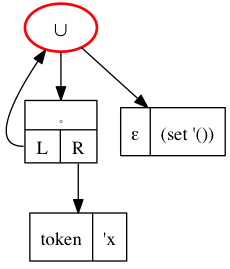
\includegraphics[width=1.5in]{xs-left-step-0.png}
 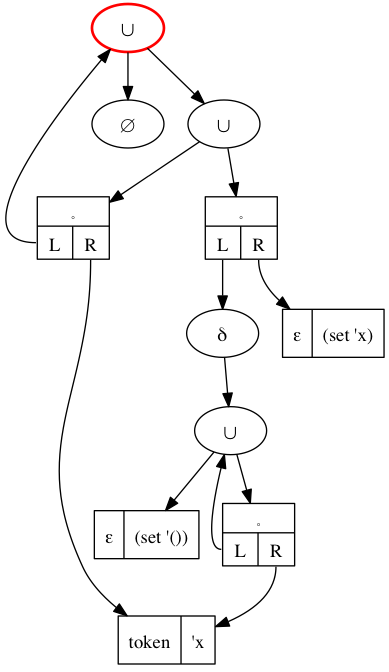
\includegraphics[width=1.5in]{xs-left-step-1.png}
 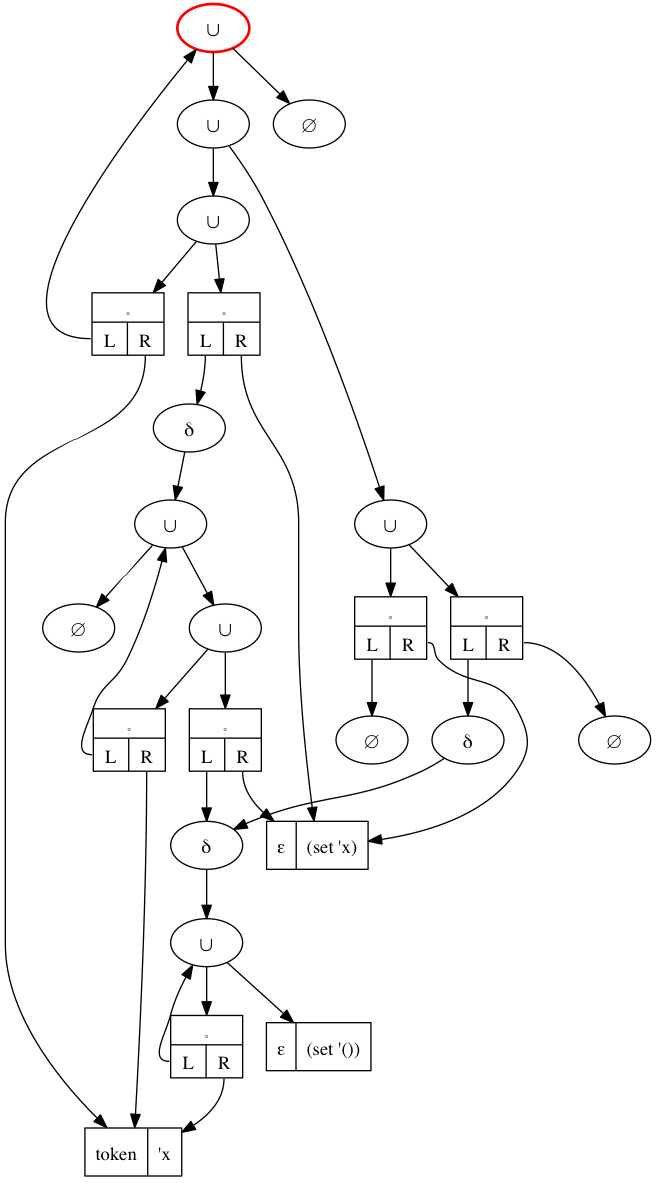
\includegraphics[width=1.5in]{xs-left-step-2.png}
\end{center}

These diagrams confirm our suspicion of exponential growth for even trivial
grammars is confirmed empirically.
%
But, smaller yet equivalent, grammars exist for the
first and second derivative.
%
That insight yields hope that we can tame the derivative.


%
Consider the fact that context-free \emph{languages}, not just grammars, are
closed under the derivative.
%
{\tt Xs-left} represents the set of all finite-length sequences of the token {\tt 'x}, and
its derivative, conceptually, is itself.
%
In the context of parsing, the derivative of {\tt xs-left} is not exactly {\tt xs-left}; the
derivative needs to remember it has seen a token through an epsilon reduction
node.
%
The \emph{intuition}, however, that the derivative should be similar in
structure to {\tt xs-left} holds strong.

For example, the following grammars are equivalent to the previously presented
first and second derivative of {\tt xs-left}:
%
\begin{center}
 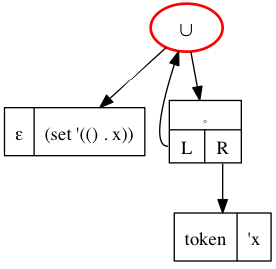
\includegraphics[width=1.5in]{xs-left-step-1-c.png}
 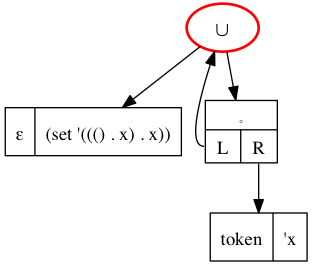
\includegraphics[width=1.5in]{xs-left-step-2-c.png}
\end{center}
%
The change is not in the language to be recognized, but in the result to be
returned through epsilon nodes.
%
In the next section we develop a theory of optimizations to find these
equivalent and more compact grammars.
  


\section{Compaction}
%
To develop the compaction optimization,
we will transform equalities on parsers into code as rewrite rules.
%
Under each rule, the resulting parser is strictly smaller.
%
We begin by writing down the equalities, and 
we use $(\To)$ in lieu of $(=)$ to emphasize direction.

First, we identify parsers which are equivalent to $\emptyset$:
%
\begin{align*}
  \emptyset \union \emptyset &\To \emptyset
  \\
  \emptyset \cat p &\To \emptyset
  \\
  p \cat \emptyset &\To \emptyset
  \\
  \emptyset \to f &\To \emptyset
  \\
  \delta(L) &\To \emptyset \text{ if } L \text{ not nullable}
\end{align*}
%
Next, parsers which are equivalent to a $\epsilon$-reduction:
%
\begin{align*}
  (\epsilon \downto S_1) \union (\epsilon \downto S_2) &\To \epsilon \downto (S_1 \union S_2)
  \\
  (\epsilon \downto S_1) \cat (\epsilon \downto S_2) &\To \epsilon \downto (S_1 \times S_2)
  \\
  (\epsilon \downto \{t_1, \ldots, t_n\}) \to f & \To \epsilon \downto
       \{ f(t_1), \ldots, f(t_n) \}
  \\
  \delta(L) &\To \epsilon \downto \lfloor L \rfloor (\epsilon) \text{ if } L \text{ is nullable}
  \\
  (\epsilon \downto S)^\star &\to \epsilon \downto (S^\star)
\end{align*}
%
And lastly, parsers equivalent under reduction or union:
%
\begin{align*}
  \emptyset \union p = p \union \emptyset &\To p
  \\
  (\epsilon \downto \set{t_1}) \cat p &\To p \to \lambda t_2 .(t_1, t_2)
  \\
  p \cat (\epsilon \downto \set{t_2}) &\To p \to \lambda t_1 .(t_1, t_2)
  \\
  (p \to f) \to g &\To p \to (g \circ f)
\end{align*}

% The equations induce  $\emptyset$ and
% $(\epsilon \downto S)$ can be generalized to the equivalence classes of
% grammars under the same equations.
% %
% This leads naturally to a fixed-point interpretation for recognition of these
% classes.
% %
% To recognize equivalence classes $\emptyset$ and $(\epsilon \downto S)$ we
% define \texttt{$\emptyset$?}:
%

To convert these compaction rules into working code, we need to be able to recognize empty parsers and null parsers:
%

%
%
\begin{code}
(define/fix (∅? p)
  #:bottom #t
  (match p
    [(∅)            #t]
    [(\ttepsred T)        (set-empty? T)]
    [(token _)      #f]

    [(δ p)          (not (nullable? p))]
    [(\ttcup p1 p2)      (and (∅? p1) (∅? p2))]
    [(∘ p1 p2)      (or  (∅? p1) (∅? p2))]
    [(\(\star\) p1)         #f]
    [(→ p1 _)      (∅? p1)]))\end{code}
 and \texttt{\ttepsilon?}:
\begin{code}
(define/fix (\ttepsilon? p)
  #:bottom #f
  (match p
    [(∅)            #f]
    [(\ttepsred _)        \,#t]
    [(token _)      #f]

    [(δ p)          (nullable? p)]
    [(\ttcup p1 p2)      (and (\ttepsilon? p1) (\ttepsilon? p2))]
    [(∘ p1 p2)      (and (\ttepsilon? p1) (\ttepsilon? p2))]
    [(\(\star\) p1)         (or  (\ttepsilon? p1) (∅? p1))]
    [(→ p1 _)      (\ttepsilon? p1)]))
\end{code}

Rolling the rewrite rules into a single function, {\tt K}, yields:
%
\begin{code}
(define/memoize (K [p #:eq])
  (match p
    [(? ∅?)                    (∅)]
    [(? \ttepsilon?)                    (\ttepsred (parse-null p))]
    [(\ttcup (? ∅?) p2)             (K p2)]
    [(\ttcup p1 (? ∅?))             (K p1)]
    [(\ttcup p1 p2)                 (\ttcup (K p1) (K p2))]
    [(∘ (singleton-\ttepsilon? e) p2)   (→ (K p2) (λ (w2) (cons e w2)))]
    [(∘ p1 (singleton-\ttepsilon? e))   (→ (K p1) (λ (w1) (cons w1 e)))]
    [(∘ p1 p2)                 (∘ (K p1) (K p2))]
    [(\(\star\) p)                     (\(\star\) (K p))]      
    [(→ (→ p f) g)           (→ (K p) (compose g f))]
    [(→ p f)                  (→ (K p) f)]
    [_                         p]))
\end{code}
%
To implement compaction, the parsing algorithm applies the function {\tt K}
after each derivative.


\subsection{Complexity}
%
The worst-case complexity of parsing under compaction is worse
than naive parsing.
%
Yet, for ``sensible'' grammars, this is not a concern.
%
We define \emph{sensible grammars} as
unambiguous, LL($k$) or LR($k$).
%
We will address generally unambiguous grammars briefly after our more targeted
narrative on sensible grammars.

The cost-model of parsing with compaction is the same as before:
\begin{align*}
  & \text{number of derivatives} 
 \\
 \times\; & \text{cost of derivative} 
 \\
 +\; & \text{cost of fixed point at the end}
 \text.
\end{align*}
%
The worst-case cost of the derivative is now cubic in the size of the current
grammar because it computes several fixed-point analyses to trigger
simplification.
%
As before, the grammar may double in size under the derivative (in the worst
case), and the cost of the fixed point at the end is negligeable.
%
The worst-case complexity of parsing under compaction is therefore:
%
\begin{equation*}
  |G|^3 + (2 \cdot |G|)^3 + (2 \cdot 2 \cdot |G|)^3 + ... = |G|^3 \sum_{i=0}^n (2^i)^3 \in O(|G|8^n)
\end{equation*}

For sensible grammars, however, we find the run-time of parsing with compaction much improved.
%
On the previously presented {\tt xs-left} example, the size of the grammar stays
constant under compaction.
%
In fact for almost every sensible gramar we have tested, compaction is able to
keep the size of the grammar nearly constant.
%
The only growth of the grammar appears when entering truly context-free portions of
the grammar, and this growth follows a stack-like structure linear in the depth of the parse tree.

Furthermore, for sensible grammars the cost of the fixed-point analysis is
constant in all of our experiments.
%
Pathalogical grammars exist which stroke the cubic worst-case runtime of the
fixed point, but we have yet to see this bad behavior appear for sensible
grammars.

We hypothesize that parsing with compaction is linear for sensible
\emph{regular} grammars.
%
The claim is supported by observing that the cost of the fixed point is constant
and the size of the grammar doesn't grow:
%
\begin{equation*}
  (K + |G|) + (K + |G|) + (K + |G|) + ... = n (K + |G|) \in O(|G| n)
\end{equation*}

We are also confident that parsing with compaction is at worst quadratic for
sensible \emph{context-free} grammars.
%
The claim is supported by observing that the cost of the fixed point is constant
and the size of the grammar grows at most by a constant factor $t$:
%
\begin{equation*}
  (K + |G|) + (K + |G| + t) + (K + |G| + 2t) + ... = n (K + |G|) + t \sum_{i=0}^n i \in O(|G| n^2)
\end{equation*}

\section{Focusing}

It is a shame that parsing with derivatives under compaction cannot be linear
for ``sensible'' \emph{context-free} grammars.
%
Quadratic parse-times for every-day context-free languages are a show-stopper
for the purported ``practicality'' of any parsing theory.
%
We present a simple grammar---nested-parentheses---which illustrates the linear
growth of a context-free grammar during parsing:
%
\begin{code}
(define parens (∪ (∘ (token 'LP) (∘ parens (token 'RP)))
                  \,(\ttepsilon (set '()))))
\end{code}

Observe the structure of {\tt parens} after zero, two and four derivatives under
compaction parsing:
%
\begin{center}
 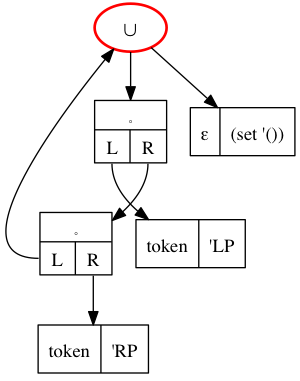
\includegraphics[width=1.5in]{parens-step-0-c.png}
 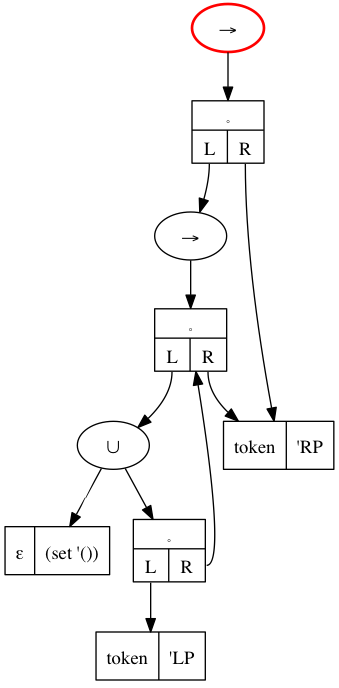
\includegraphics[width=1.5in]{parens-step-2-c.png}
 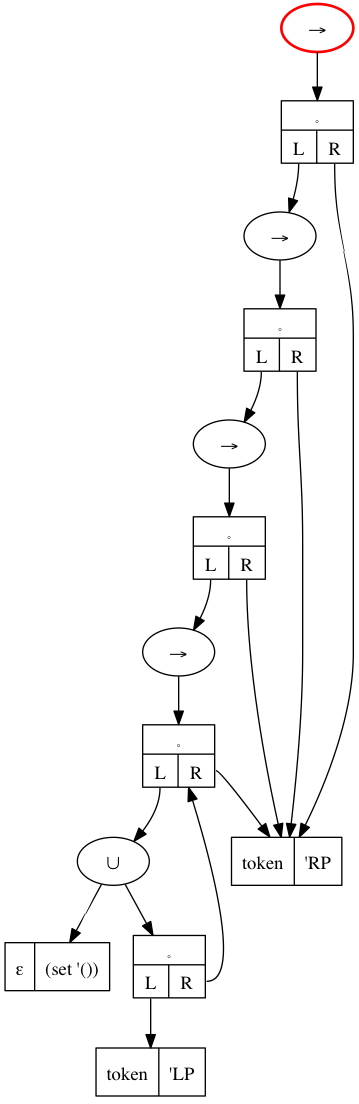
\includegraphics[width=1.5in]{parens-step-4-c.png}
\end{center}

The grammar grows linearly as it retains a stack for the context-free portion
of the grammar.
%
In this section we manage this growth through yet another equational theory,
bringing the cost of derivative parsing down to linear for ``sensible''
grammars in practice.

We introduce the following equations for the derivative, which follow trivially
from definition:
%
\begin{align*}
  D_c(L_1 \cat L_2) &= L_1 \cat D_c(L_2) & &\text{ if } L_1 = \epsilon
  \\
  D_c(L_1 \cat L_2) &= D_c(L_1) \cat L_2 & &\text{ if } L_1 \text{ not nullable}
  \\
  D_c(L \to f) &= D_c(L) \to f
\end{align*}
%
[We note that other equations exist, but these are the only three which aren't
subsumed by compaction.]

With the above equations, the ``focus'' of the derivative can be repositioned
through concatenation and reduction connectives to a smaller sub-grammar, given
that certain conditions hold.
%
In the {\tt parens} example, the focus of the derivative can be repositioned through
the entire growth portion of the grammar:
%
\begin{center}
 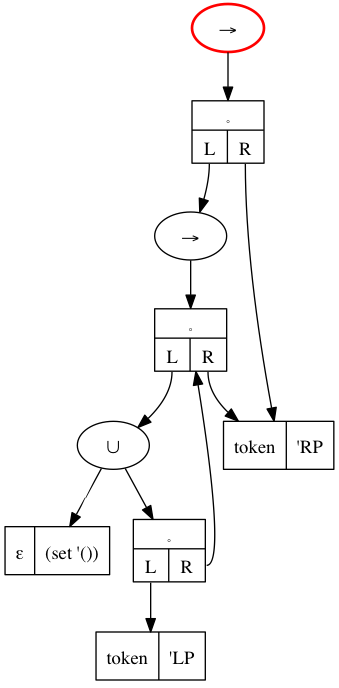
\includegraphics[width=1.5in]{parens-step-2-c.png}
 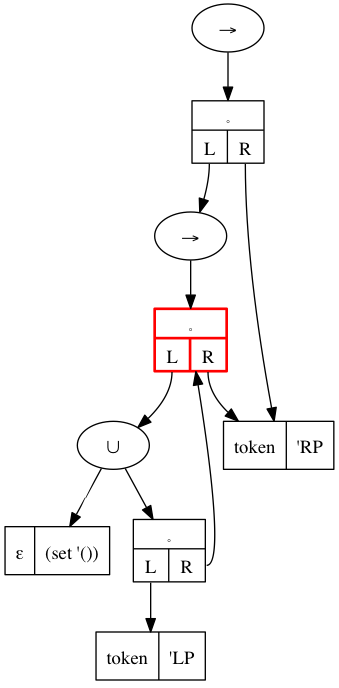
\includegraphics[width=1.5in]{parens-step-2-f.png}
\end{center}
%
The derivative equations justify the focusing; taking the derivative on the
focused grammar yeilds the same result as taking the derivative on the whole.

\subsection{Zippers}
To represent a focused grammar we use a functional zipper datatype for the
grammar.
%
A top-level zipper parser is now represented as a parser and a context, where
the top-level zipper parser \emph{does not} occur recursively inside the
parser.
%
The context type is the \emph{datatype derivative} of the parser type.
%
Because we only introduced equations for concatentation and reduction, we only
include their datatype derivatives:
%
\begin{code}
(define-struct zipper {parser context})
  
(define-struct \(\Box\cat\bullet\) {L2 k}) ; \(\cat\) with a missing left parser
(define-struct \(\bullet\cat\Box\) {L1 k}) ; \(\cat\) with a missing right parser
(define-struct \(\Box\to\bullet\) {L k})  ; \(\to\) with a missing parser
\end{code}

The interpretation of a zipper---pzip---fills the hole of a context with a
parser:
\begin{code}
(define (pzip Z)
  (match Z
    [(zipper L 'top)           L]
    [(zipper L1 (\(\Box\cat\bullet\) L2 k))  (pzip (zipper (∘ L1 L2) k))]
    [(zipper L2 (\(\bullet\cat\Box\) L1 k))  (pzip (zipper (∘ L1 L2) k))]
    [(zipper L (\(\Box\to\bullet\) f k))   (pzip (zipper (→ L f) k))]))
\end{code}

Finally we follow the derivative equations to write a procedure---drill---which
constructs a zipper by focusing on the inner-most relevant derivative
position:
\begin{code}
(define (drill Z)
  (match Z
    [(zipper L k)
     (match L
       [(\(\cat\) (? essentially-ε? L1) 
           (and (not (? essentially-ε?)) L2)) 
        ; \(\To\)
        (drill (zipper L2 (\(\bullet\cat\Box\) L1 k)))]
       [(\(\cat\) (and L1 (not (? nullable?))) L2) 
        ; \(\To\)
        (drill (zipper L1 (\(\Box\cat\bullet\) L2 k)))]
       [(\(\to\) (and (not (? essentially-ε?)) L) f) 
        ; \(\To\)
        (drill (zipper L (\(\Box\to\bullet\) f k)))]
       [_                                            
        ; \(\To\)
        Z])]))
\end{code}
%
[Note: ``(and (not (? essentiall-ε?)) L)'' is a Racket matching pattern for
``if essentially-ε? returns false then match and bind to L''.]
 
We remark that drill has the following property:
%
\begin{code}
drill p = (zipper p' k) \(\implies\) 
  D_c(p) = D_c(pzip p' k) = pzip D_c(p') k
\end{code}

We are not yet able to use drill in a new parsing algorithm.
%
After drilling and performing a derivative on the focused grammar, it is
possible that the resulting grammar has become nullable.
%
Nullability of the resulting grammar may violate the second derivative equation
for some concatentation node in the context, rendering the next derivative step
on the focused grammar unsound.
%
Our last procedure, regress, backs out of nullable parsers:
\begin{code}
(define (regress Z)
  (match Z
    [(zipper (? nullable? L1) (\(\Box\cat\bullet\) L2 k))   
     ; \(\To\)
     (regress (zipper (\(\cat\) L1 L2) k))]
    [(zipper (? nullable? L2) (\(\bullet\cat\Box\) L1 k))
     ; \(\To\)
     (regress (zipper (\(\cat\) L1 L2) k))]
    [(zipper (? nullable? L1) (\(\Box\to\bullet\) f k))    
     ; \(\To\)
     (regress (zipper (\(\to\) L1 f) k))]
    [(zipper L k)
     ; \(\To\)
     Z]))
\end{code}

\subsection{Algorithm}
The completed focusing algorithm, and our final optimization for derivative
parsing, consists of the sequence: derive, compact, regress, drill.
%
Rinse and repeat.
%
We present images of the parentheses grammar parsing the input '(LP LP RP RP)
to supplement understanding of drilling and regression:
%
\begin{center}
 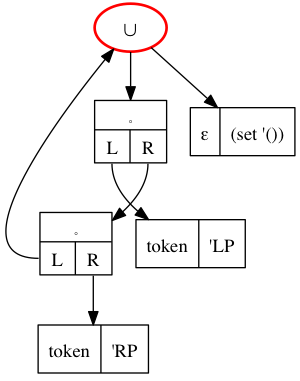
\includegraphics[width=1.5in]{parens-short-step-0-f.png}
 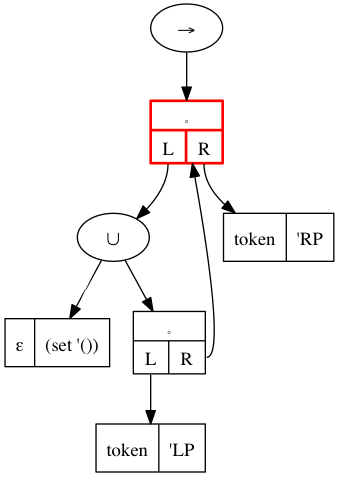
\includegraphics[width=1.5in]{parens-short-step-1-f.png}
 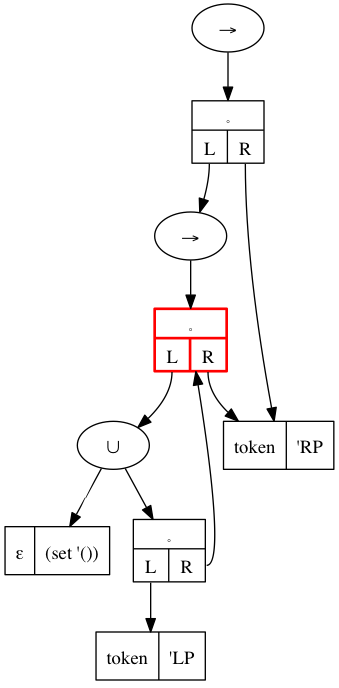
\includegraphics[width=1.5in]{parens-short-step-2-f.png}
 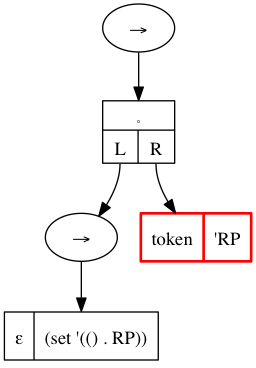
\includegraphics[width=1.5in]{parens-short-step-3-f.png}
 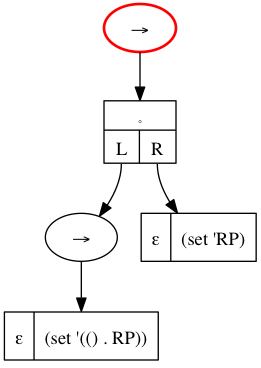
\includegraphics[width=1.5in]{parens-short-step-4-f.png}
\end{center}

\subsection{Complexity}

With focusing we are able to keep the subject of the derivative operation
constant, and our argument for linear parsing complexity on ``sensible''
grammars is repeated.
%
Parsing with derivatives can be practical provided two optimizations,
compaction and focusing.

To see where focusing is unable to keep parsing time linear for unambiguous but
non-LR(k) (and therefore non-``sensible'') grammars we present
the after-parens grammar:
\begin{code}
  (define after-parens
    (∪ a-after-parens b-after-parens))
  (define a-after-parens (∘ parens (token 'a)))
  (define b-after-parens (∘ parens (token 'b)))
\end{code}
%
The grammar is unambiguous; a successfull parse comes from exactly one
derivation.
%
However there is nontrivial ambiguity during parsing: a parser does not know which
branch of {\tt a-after-parens} or {\tt b-after-parens} to take until the very end.
%
It is through this ambiguity during parsing that after-parens violates LL(k) or
LR(k); no k exists under which the branch can always be predicted.
%
Let's observe how parsing with derivatives under focusing looks after zero, two,
and four derivatives:
%
\begin{center}
 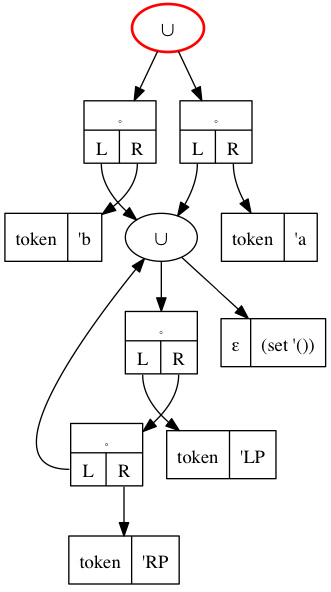
\includegraphics[width=1.5in]{after-parens-step-0-f.png}
 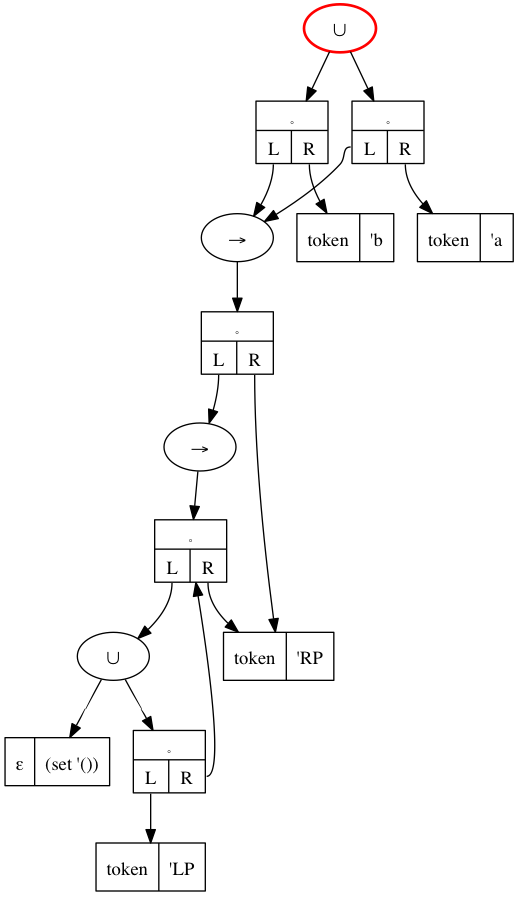
\includegraphics[width=1.5in]{after-parens-step-2-f.png}
 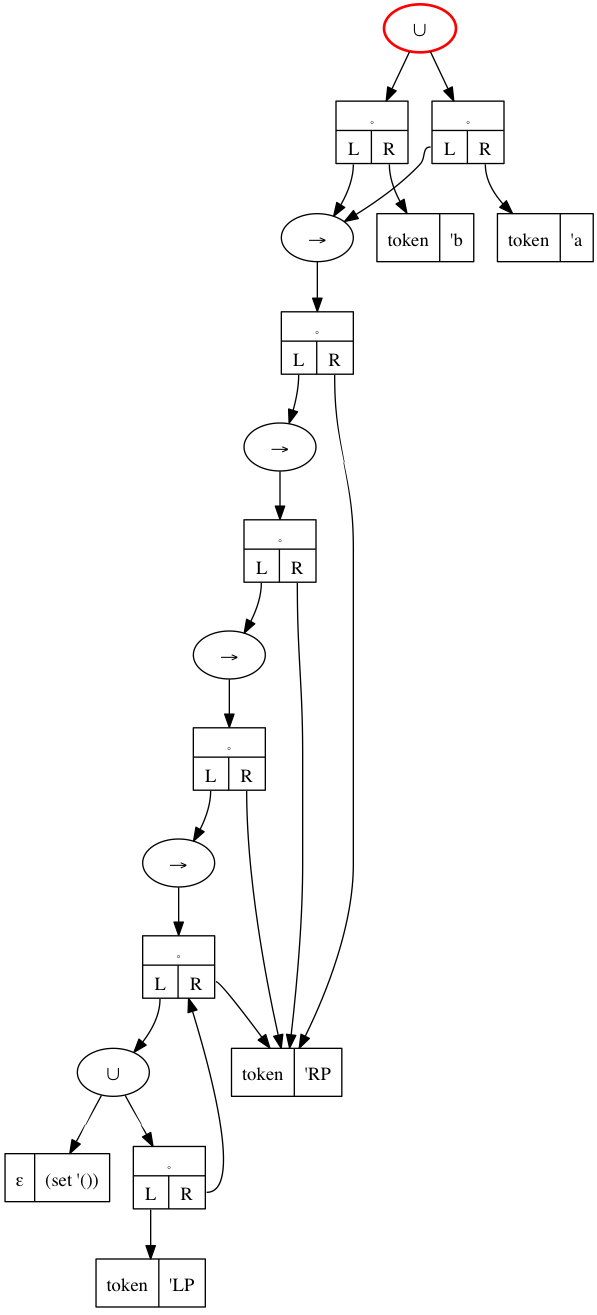
\includegraphics[width=1.5in]{after-parens-step-4-f.png}
\end{center}
%
The ambiguity during parsing blocks the zipper algorithm from focusing through
the growth of grammar and the size grows linearly with the input.
%
Our algorithm is therefore quadratic when parsing after-parens.

We can imagine yet another optimization which includes zippers \emph{as a
proper parser connective}, allowing parsers to recursively contain zipper
parsers.
%
In theory this would allow drill to dive through nested contexts, not just
those at the top-level, keeping the size of after-parens constant during
parsing.
%
However, this addition to the algebra complicates the derivative and other
analysis theories, and we leave its development for future work.

\subsection{Complexity Conjectures vs Proofs}

We do not given full proof of our complexity conjectures because they are just
that: conjectures.
%
A proof of complexity on LR(k) languages would involve relating our algorithm
to LR(k) grammars, which are defined entirely be the shift/reduce tables which
LR parsing algorithms generate.
%
Relating the derivative to shift/reduce tables would be tiresome.
%
However, we believe there is a class of grammars, similar to LR(k) but defined
in terms of derivatives, for which parsing with derivatives under focusing
\emph{is} provably linear.
%
We leave such a proof for future work, and merely present our preliminary
empirical results: we have yet to find an unambiguous LL(k) or LR(k) grammar
that our algorithm cannot parse in linear time.

\section{Related work}

There has been a revival of interest in Brzozowski's derivative, itself a
specialization of the well-known left quotient operation on languages.
%
Owens, Reppy and Turon re-examined the derivative in light of lexer
construction~\cite{mattmight:Owens:2009:Derivative}, and
Danielsson~\cite{mattmight:Danielsson:2010:Total} used it to prove the totality
of parser combinators.


The literature on parsing is vast;
there are dozens of methods for parsing, including but not limited to
abstract interpretation~\cite{mattmight:Cousot:2003:Parsing,mattmight:Cousot:2006:Parsing},
operator-precedence parsing~\cite{mattmight:Floyd:1963:Syntactic,mattmight:Pratt:1973:TopDown},
simple precedence parsing~\cite{mattmight:Dijkstra:1982:ShuntingYard},
% bounded context parsing~\cite{mattmight:Floyd:1964:Bounded}, 
parser combinators~\cite{mattmight:Swierstra:1998:Combinator,mattmight:Swierstra:2009:Tutorial},
LALR parsing~\cite{mattmight:DeRemer:1969:LALR}, 
LR($k$) parsing~\cite{mattmight:Knuth:1965:LR},
GLR parsing~\cite{mattmight:Masaru:1984:GLR},
CYK parsing~\cite{mattmight:Kasami:1965:CYK,mattmight:Younger:1967:CYK,mattmight:Cocke:1970:CYK},
Earley parsing~\cite{mattmight:Earley:1970:Parsing},
LL($k$) parsing, and
recursive descent parsing~\cite{mattmight:Wirth:1996:CompilerConstruction}.
packrat/PEG parsing~\cite{mattmight:Ford:2002:Packrat,mattmight:Warth:2008:PEG}.
%
Derivative-based parsing shares full coverage of all context-free
grammars with GLR, CYK and Earley.

Derivative-based parsing 
is not easy to classify as a top-down or bottom-up method.
%
In personal correspondence, Stuart Kurtz
pointed out that when the grammar is in Greibach Normal Form (GNF),
the algorithm acquires a ``parallel'' top-down flavor.
%
For grammars outside GNF, while watching the algorithm evolve under compaction,
one sees what appears to be a pushdown stack emerge inside the grammar.
%
(Pushes and pops appear as the jagged edges in the graph to the left.)

The most directly related work is Danielsson's work on total parser
combinators~\cite{mattmight:Danielsson:2010:Total}.
%
His work computes residual parsers similar to our own, but does not detail a
simplification operation.
%
According to our correspondence with Danielsson, simplification does exist in
the implementation.
%
Yet, because it is unable to memoize the simplification operation (turning it
into compaction), the implementation exhibits exponential performance even in
practice.
%
This does not detract from Danielsson's contribution, which highlights the
theoretical elegance and convenience of reasoning about residual parsers.


\paragraph{Acknowledgements} 
We are grateful for the thousands of comments on
reddit, hackernews, Lambda the Ultimate and elsewhere that thoroughly
dissected and improved an earlier draft of this work.
%
We also thank the ICFP 2011 and the ESOP 2010 reviewers for their thoughtful and detailed feedback.
%
This research is partly supported by the National Science
Foundation under Grant No. 1035658, 
by the DARPA CRASH project ``GnoSys: Raising the level of discourse in systems program,''
and by the National Nuclear Security Administration under 
the ``Accelerating Development of Retorfitable CO2 Capture Technologies through Predictivity'' project
through DOE Cooperative Agreement 
DE-NA0000740.


\section{Conclusion} 
Our goal was a means
to abbreviate the understanding and
implementation of parsing.
%
Brzozowski's derivative met the challenge:
its theory is equational, 
its implementation is functional
 and, with an orthogonal optimization,
its performance is not unreasonable.


